\documentclass[11pt,oneside]{article}
\usepackage[T1]{fontenc}
\usepackage[utf8]{inputenc}
% \usepackage{lmodern}
%\usepackage[adobe-utopia,uppercase=upright,greeklowercase=upright]{mathdesign}
\usepackage[adobe-utopia]{mathdesign}
%\usepackage{minionpro}
% \usepackage{pifont}
% \usepackage{amssymb}
\usepackage{amsmath}
\usepackage[francais]{babel}
% \usepackage[francais]{varioref}
\usepackage[dvips]{graphicx}

\usepackage{framed}
\usepackage[normalem]{ulem}
\usepackage{fancyhdr}
\usepackage{titlesec}
\usepackage{vmargin}
\usepackage{longtable}

\usepackage{ifthen}


%\usepackage{epsfig}
\usepackage{subfig}

\usepackage{multirow}
\usepackage{multicol} % Portions de texte en colonnes
\usepackage{flafter}%floatants après la référence



\usepackage{color}
\usepackage{colortbl}


\definecolor{gris25}{gray}{0.75}
\definecolor{bleu}{RGB}{18,33,98}
\definecolor{bleuf}{RGB}{42,94,171}
\definecolor{bleuc}{RGB}{231,239,247}
\definecolor{rougef}{RGB}{185,18,27}
\definecolor{rougec}{RGB}{255,230,231}
\definecolor{vertf}{RGB}{103,126,82}
\definecolor{vertc}{RGB}{220,255,191}

\newenvironment{rem}[1][\hsize]%
{%
    \def\FrameCommand
    {%
\rotatebox{90}{\textit{\textsf{Remarque}}} 
        {\color{bleuf}\vrule width 3pt}%
        \hspace{0pt}%must no space.
        \fboxsep=\FrameSep\colorbox{bleuc}%
    }%
    \MakeFramed{\hsize#1\advance\hsize-\width\FrameRestore}%
}%
{\endMakeFramed}%


\newenvironment{savoir}[1][\hsize]%
{%
    \def\FrameCommand
    {%
\rotatebox{90}{\textit{\textsf{Savoir}}} 
        {\color{bleuf}\vrule width 3pt}%
        \hspace{0pt}%must no space.
        \fboxsep=\FrameSep\colorbox{bleuc}%
    }%
    \MakeFramed{\hsize#1\advance\hsize-\width\FrameRestore}%
}%
{\endMakeFramed}%

\newenvironment{prob}[1][\hsize]%
{%
    \def\FrameCommand%
    {%
\rotatebox{90}{\textit{\textsf{ Problématique}}} 
        {\color{rougef}\vrule width 3pt}%
        \hspace{0pt}%must no space.
        \fboxsep=\FrameSep\colorbox{rougec}%
    }%
    \MakeFramed{\hsize#1\advance\hsize-\width\FrameRestore}%
}%
{\endMakeFramed}%

\newenvironment{obj}[1][\hsize]%
{%
    \def\FrameCommand%
    {%
\rotatebox{90}{\textit{\textsf{ $\;$}}} 
        {\color{rougef}\vrule width 3pt}%
        \hspace{0pt}%must no space.
        \fboxsep=\FrameSep\colorbox{rougec}%
    }%
    \MakeFramed{\hsize#1\advance\hsize-\width\FrameRestore}%
}%
{\endMakeFramed}%

\newenvironment{defi}[1][\hsize]%
{%
    \def\FrameCommand%
    {%
\rotatebox{90}{\textit{\textsf{Définition\\}}} 
        {\color{bleuf}\vrule width 3pt}%
        \hspace{0pt}%must no space.
        \fboxsep=\FrameSep\colorbox{bleuc}%
    }%
    \MakeFramed{\hsize#1\advance\hsize-\width\FrameRestore}%
}%
{\endMakeFramed}%


\newenvironment{hypo}[1][\hsize]%
{%
    \def\FrameCommand%
    {%
\rotatebox{90}{\textit{\textsf{Hypothèse\\}}} 
        {\color{bleuf}\vrule width 3pt}%
        \hspace{0pt}%must no space.
        \fboxsep=\FrameSep\colorbox{bleuc}%
    }%
    \MakeFramed{\hsize#1\advance\hsize-\width\FrameRestore}%
}%
{\endMakeFramed}%


\newenvironment{prop}[1][\hsize]%
{%
    \def\FrameCommand%
    {%
\rotatebox{90}{\textit{\textsf{Propriété\\}}} 
        {\color{bleuf}\vrule width 3pt}%
        \hspace{0pt}%must no space.
        \fboxsep=\FrameSep\colorbox{bleuc}%
    }%
    \MakeFramed{\hsize#1\advance\hsize-\width\FrameRestore}%
}%
{\endMakeFramed}%

\newenvironment{props}[1][\hsize]%
{%
    \def\FrameCommand%
    {%
\rotatebox{90}{\textit{\textsf{Propriétés\\}}} 
        {\color{bleuf}\vrule width 3pt}%
        \hspace{0pt}%must no space.
        \fboxsep=\FrameSep\colorbox{bleuc}%
    }%
    \MakeFramed{\hsize#1\advance\hsize-\width\FrameRestore}%
}%
{\endMakeFramed}%

\newenvironment{exemple}[1][\hsize]%
{%
    \def\FrameCommand%
    {%
\rotatebox{90}{\textit{\textsf{Exemple\\}}} 
        {\color{vertf}\vrule width 3pt}%
        \hspace{0pt}%must no space.
        \fboxsep=\FrameSep\colorbox{vertc}%
    }%
    \MakeFramed{\hsize#1\advance\hsize-\width\FrameRestore}%
}%
{\endMakeFramed}%

\newenvironment{resultat}[1][\hsize]%
{%
    \def\FrameCommand%
    {%
\rotatebox{90}{\textit{\textsf{Résultat\\}}} 
        {\color{rougef}\vrule width 3pt}%
        \hspace{0pt}%must no space.
        \fboxsep=\FrameSep\colorbox{rougec}%
    }%
    \MakeFramed{\hsize#1\advance\hsize-\width\FrameRestore}%
}%
{\endMakeFramed}%

\newenvironment{methode}[1][\hsize]%
{%
    \def\FrameCommand%
    {%
\rotatebox{90}{\textit{\textsf{Méthode\\}}} 
        {\color{rougef}\vrule width 3pt}%
        \hspace{0pt}%must no space.
        \fboxsep=\FrameSep\colorbox{rougec}%
    }%
    \MakeFramed{\hsize#1\advance\hsize-\width\FrameRestore}%
}%
{\endMakeFramed}%

\newenvironment{theo}[1][\hsize]%
{%
    \def\FrameCommand%
    {%
\rotatebox{90}{\textit{\textsf{Théorème\\}}} 
        {\color{rougef}\vrule width 3pt}%
        \hspace{0pt}%must no space.
        \fboxsep=\FrameSep\colorbox{rougec}%
    }%
    \MakeFramed{\hsize#1\advance\hsize-\width\FrameRestore}%
}%
{\endMakeFramed}%

\newenvironment{warn}[1][\hsize]%
{%
    \def\FrameCommand%
    {%
\rotatebox{90}{\textit{\textsf{Attention\\}}} 
        {\color{rougef}\vrule width 3pt}%
        \hspace{0pt}%must no space.
        \fboxsep=\FrameSep\colorbox{rougec}%
    }%
    \MakeFramed{\hsize#1\advance\hsize-\width\FrameRestore}%
}%
{\endMakeFramed}%

% \usepackage{pstricks}
%\usepackage{minitoc}
% \setcounter{minitocdepth}{4}

\setcounter{tocdepth}{2}

% \mtcselectlanguage{french} 

%\usepackage{draftcopy}% "Brouillon"
% \usepackage{floatflt}
\usepackage{psfrag}
%\usepackage{listings} % Permet d'insérer du code de programmation
\renewcommand{\baselinestretch}{1.2}

% Changer la numérotation des figures :
% ------------------------------------
% \makeatletter
% \renewcommand{\thefigure}{\ifnum \c@section>\z@ \thesection.\fi
%  \@arabic\c@figure}
% \@addtoreset{figure}{section}
% \makeatother
 


%%%%%%%%%%%%
% Définition des vecteurs %
%%%%%%%%%%%%
 \newcommand{\vect}[1]{\overrightarrow{#1}}

%%%%%%%%%%%%
% Définition des torseusr %
%%%%%%%%%%%%

 \newcommand{\torseur}[1]{%
\left\{{#1}\right\}
}

\newcommand{\torseurcin}[3]{%
\left\{\mathcal{#1} \left(#2/#3 \right) \right\}
}

\newcommand{\torseurstat}[3]{%
\left\{\mathcal{#1} \left(#2\rightarrow #3 \right) \right\}
}

 \newcommand{\torseurc}[8]{%
%\left\{#1 \right\}=
\left\{
{#1}
\right\}
 = 
\left\{%
\begin{array}{cc}%
{#2} & {#5}\\%
{#3} & {#6}\\%
{#4} & {#7}\\%
\end{array}%
\right\}_{#8}%
}

 \newcommand{\torseurcol}[7]{
\left\{%
\begin{array}{cc}%
{#1} & {#4}\\%
{#2} & {#5}\\%
{#3} & {#6}\\%
\end{array}%
\right\}_{#7}%
}

 \newcommand{\torseurl}[3]{%
%\left\{\mathcal{#1}\right\}_{#2}=%
\left\{%
\begin{array}{l}%
{#1} \\%
{#2} %
\end{array}%
\right\}_{#3}%
}

 \newcommand{\vectv}[3]{%
\vect{V\left( {#1} \in {#2}/{#3}\right)}
}


\newcommand{\vectf}[2]{%
\vect{R\left( {#1} \rightarrow {#2}\right)}
}

\newcommand{\vectm}[3]{%
\vect{\mathcal{M}\left( {#1}, {#2} \rightarrow {#3}\right)}
}


 \newcommand{\vectg}[3]{%
\vect{\Gamma \left( {#1} \in {#2}/{#3}\right)}
}

 \newcommand{\vecto}[2]{%
\vect{\Omega\left( {#1}/{#2}\right)}
}
% }$$\left\{\mathcal{#1} \right\}_{#2} =%
% \left\{%
% \begin{array}{c}%
%  #3 \\%
%  #4 %
% \end{array}%
% \right\}_{#5}}

%  ------------------------------------------
% | Modification du formatage des sections : | 
%  ------------------------------------------

% Grands titres :
% ---------------

\newcommand{\titre}[1]{%
\begin{center}
      \bigskip
      \rule{\textwidth}{1pt}
      \par\vspace{0.1cm}
      
      \textbf{\large #1}
      \par\rule{\textwidth}{1pt}
    \end{center}
    \bigskip
  }

% Supprime le numéro du chapitre dans la numérotation des sections:
% -----------------------------------------------------------------
\makeatletter
\renewcommand{\thesection}{\@arabic\c@section}
\makeatother


% \titleformat{\chapter}[display]
% {\normalfont\Large\filcenter}
% {}
% {1pc}
% {\titlerule[1pt]
%   \vspace{1pc}%
%   \Huge}[\vspace{1ex}%
% \titlerule]


%%%% Chapitres Comme PY Pechard %%%%%%%%%
% numéro du chapitre
\DeclareFixedFont{\chapnumfont}{OT1}{phv}{b}{n}{80pt}
% pour le mot « Chapitre »
\DeclareFixedFont{\chapchapfont}{OT1}{phv}{m}{it}{40pt}
% pour le titre
\DeclareFixedFont{\chaptitfont}{T1}{phv}{b}{n}{25pt}

\definecolor{gris}{gray}{0.75}
\titleformat{\chapter}[display]%
	{\sffamily}%
	{\filleft\chapchapfont\color{gris}\chaptertitlename\
	\\
	\vspace{12pt}
	\chapnumfont\thechapter}%
	{16pt}%
	{\filleft\chaptitfont}%
	[\vspace{6pt}\titlerule\titlerule\titlerule]

%%%%  Fin Chapitres Comme PY Pechard %%%%%%%%%


% Section, subsection, subsubsection sans serifs :
% % ----------------------------------------------

% \makeatletter
% \renewcommand{\section}{\@startsection{section}{0}{0mm}%
% {\baselineskip}{.3\baselineskip}%
% {\normalfont\sffamily\Large\textbf}}%
% \makeatother

\makeatletter
\renewcommand{\@seccntformat}[1]{{\textcolor{bleu}{\csname
the#1\endcsname}\hspace{0.5em}}}
\makeatother

\makeatletter
\renewcommand{\section}{\@startsection{section}{1}{\z@}%
                       {-4ex \@plus -1ex \@minus -.4ex}%
                       {1ex \@plus.2ex }%
                       {\normalfont\Large\sffamily\bfseries}}%
\makeatother
 
\makeatletter
\renewcommand{\subsection}{\@startsection {subsection}{2}{\z@}
                          {-3ex \@plus -0.1ex \@minus -.4ex}%
                          {0.5ex \@plus.2ex }%
                          {\normalfont\large\sffamily\bfseries}}
\makeatother
 
\makeatletter
\renewcommand{\subsubsection}{\@startsection {subsubsection}{3}{\z@}
                          {-2ex \@plus -0.1ex \@minus -.2ex}%
                          {0.2ex \@plus.2ex }%
                          {\normalfont\large\sffamily\bfseries}}
\makeatother
 
\makeatletter             
\renewcommand{\paragraph}{\@startsection{paragraph}{4}{\z@}%
                                    {-2ex \@plus-.2ex \@minus .2ex}%
                                    {0.1ex}%               
{\normalfont\sffamily\bfseries}}
\makeatother
 
\makeatletter
\renewcommand{\subparagraph}{\@startsection{subparagraph}{5}{\z@}%
                                       {-2ex \@plus-.1ex \@minus .2ex}%
                                       {0.1ex}%
				    {\normalfont\normalsize\sffamily\bfseries}}
\makeatletter
% \makeatletter
% \renewcommand{\subsection}{\@startsection{subsection}{1}{2mm}%
% {\baselineskip}{.3\baselineskip}%
% {\normalfont\sffamily\large\textbf}}%
% \makeatother
% 
% \makeatletter
% \renewcommand{\subsubsection}{\@startsection{subsubsection}{2}{4mm}%
% {\baselineskip}{.15\baselineskip}%
% {\normalfont\sffamily\large\textbf}}%
% \makeatother
% 
% \makeatletter
% \renewcommand{\paragraph}{\@startsection{paragraph}{3}{6mm}%
% {\baselineskip}{.15\baselineskip}%
% {\normalfont\sffamily\large\textbf}}%
% \makeatother
 
\setcounter{secnumdepth}{4}


%  --------
% | Marges |
%  --------


% \setmarginsrb{2.5cm}{1.5cm}{2.5cm}{2cm}{1cm}{1cm}{1cm}{1cm}
\setmarginsrb{1.5cm}{1cm}{1cm}{1.5cm}{1cm}{1cm}{1cm}{1cm}

% Changer les marges localement :
% -----------------------------
\newenvironment{changemargin}[2]{\begin{list}{}{%
\setlength{\topsep}{0pt}%
\setlength{\leftmargin}{0pt}%
\setlength{\rightmargin}{0pt}%
\setlength{\listparindent}{\parindent}%
\setlength{\itemindent}{\parindent}%
\setlength{\parsep}{0pt plus 1pt}%
\addtolength{\leftmargin}{#1}%
\addtolength{\rightmargin}{#2}%
}\item }{\end{list}}



\usepackage{pst-solides3d}
\usepackage{titletoc}
\titlecontents{chapter}[+3pc]
  {\addvspace{10pt}\sffamily\bfseries}
{\contentslabel[{\pscirclebox[fillstyle=solid,fillcolor=gray!25,
linecolor=gray!25,framesep=4pt]{\textcolor{white}{\thecontentslabel}}}]{2.5pc}}
  {}
  {\dotfill \normalfont\thecontentspage\ }

\titlecontents{section}[3pc]
  {\addvspace{2pt}\sffamily}
  {\contentslabel[\thecontentslabel]{1.8pc}}
  {}
  {\dotfill \normalfont\thecontentspage\ }

\titlecontents{subsection}[5pc]
  {\addvspace{2pt}\sffamily}
  {\contentslabel[\thecontentslabel]{1.8pc}}
  {}
  {\dotfill \normalfont\thecontentspage\ }

\titlecontents{subsubsection}[8pc]
  {\addvspace{2pt}\sffamily}
  {\contentslabel[\thecontentslabel]{3pc}}
  {}
  {\dotfill \normalfont\thecontentspage\ }
%{\;\titlerule\;\normalfont\thecontentspage\ }

\titlecontents{paragraph}[9pc]
  {\addvspace{2pt}\sffamily}
  {\contentslabel[\thecontentslabel]{3.5pc}}
  {}
  {\dotfill \normalfont\thecontentspage\ }



\usepackage[raccourcis]{FAST}
\usepackage[%
    pdftitle={Produits Procédés Matériaux -- },
    pdfauthor={Xavier Pessoles},
    colorlinks=true,
    linkcolor=blue,
    citecolor=magenta]{hyperref}

\usepackage{pifont}


% \makeatletter \let\ps@plain\ps@empty \makeatother
%% DEBUT DU DOCUMENT
%% =================
\sloppy
\hyphenpenalty 10000

\newcommand{\Pointilles}[1][3]{%
\multido{}{#1}{\makebox[\linewidth]{\dotfill}\\[\parskip]
}}


\colorlet{shadecolor}{orange!15}

\newtheorem{theorem}{Theorem}


\begin{document}


\newboolean{prof}
\setboolean{prof}{true}
%------------- En tetes et Pieds de Pages ------------
\pagestyle{fancy}
\renewcommand{\headrulewidth}{0pt}

\fancyhead{}
\fancyhead[L]{%
\noindent\noindent\begin{minipage}[c]{2.6cm}
%Lycée Rouvière PTSI

\includegraphics[width=2cm]{png/logo_ptsi.png}%
\end{minipage}
}

\fancyhead[C]{\rule{12cm}{.5pt}}

\fancyhead[R]{%
\noindent\begin{minipage}[c]{3cm}
\begin{flushright}
\footnotesize{\textit{\textsf{Sciences Industrielles\\ pour l'Ingénieur}}}%
\end{flushright}
\end{minipage}
}

\renewcommand{\footrulewidth}{0.2pt}

\fancyfoot[C]{\footnotesize{\bfseries \thepage}}
\fancyfoot[L]{\footnotesize{2012 -- 2013} \\ X. \textsc{Pessoles}}
\ifthenelse{\boolean{prof}}{%
\fancyfoot[R]{\footnotesize{Cours -- CI 6 : PPM -- P}}
}{%
\fancyfoot[R]{\footnotesize{Cours -- CI 6 : PPM}}
}



\begin{center}
 \huge\textsc{CI 6 -- PPM -- Produits Procédés Matériaux}

 \large\textsc{Élaboration des pièces mécaniques. Introduction de la chaîne numérique.}
\end{center}

\begin{center}
 \LARGE\textsc{Chapitre 7 -- Spécifications des ajustements entre arbres et moyeux}
\end{center}

%\begin{flushright}
%\textit{D'après documents de Jean-Pierre Pupier}
%\end{flushright}

\vspace{.5cm}



%\begin{minipage}[c]{.3\linewidth}
%\begin{center}
%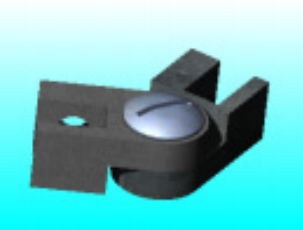
\includegraphics[height=2.5cm]{png/charniere1}

%\textit{Produit désiré par l'utilisateur}
%\end{center}
%\end{minipage} \hfill
%\begin{minipage}[c]{.3\linewidth}
%\begin{center}
%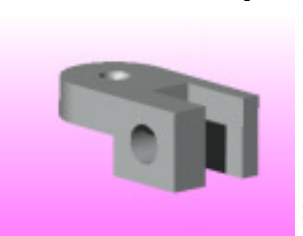
\includegraphics[height=2.5cm]{png/charniere2}

%\textit{Produit issu de la conception}
%\end{center}
%\end{minipage} \hfill
%\begin{minipage}[c]{.3\linewidth}
%\begin{center}
%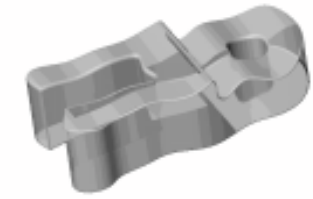
\includegraphics[height=2.5cm]{png/charniere3}

%\textit{Produit issu de la fabrication}
%\end{center}
%\end{minipage}

%\vspace{.5cm}

Dans le cadre de la conception de systèmes mécaniques, il est très courant d'avoir des contacts de type arbre -- moyeu, les arbres ou les moyeux pouvant être à section circulaire ou rectangulaire. Les surfaces étant en contact, un seul trait est visible dans le dessin de définition. Cependant, suivant les contraintes fonctionnelles, on peut désirer qu'il y ait un glissement entre les surfaces ou au contraire un blocage.

La spécification d'ajustements sur les dessins de définition permettent de savoir si un assemblage est serré, incertain ou glissant. Lors de l'assemblage ou de la maintenance du mécanisme on s'attachera à ce que les pièces soient \textbf{interchangeables}, c'est-à-dire qu'une pièce sera échangeable avec n'importe quelle autre pièce étant conforme. Dans le cas où les contraintes dimensionnelles seront trop fortes, il faudra avoir recours à \textbf{l'appairage} : dans ce cas, il faudra pré - associer 2 ou plus de pièces afin d'assurer l'assemblage du système.




%\begin{center}
%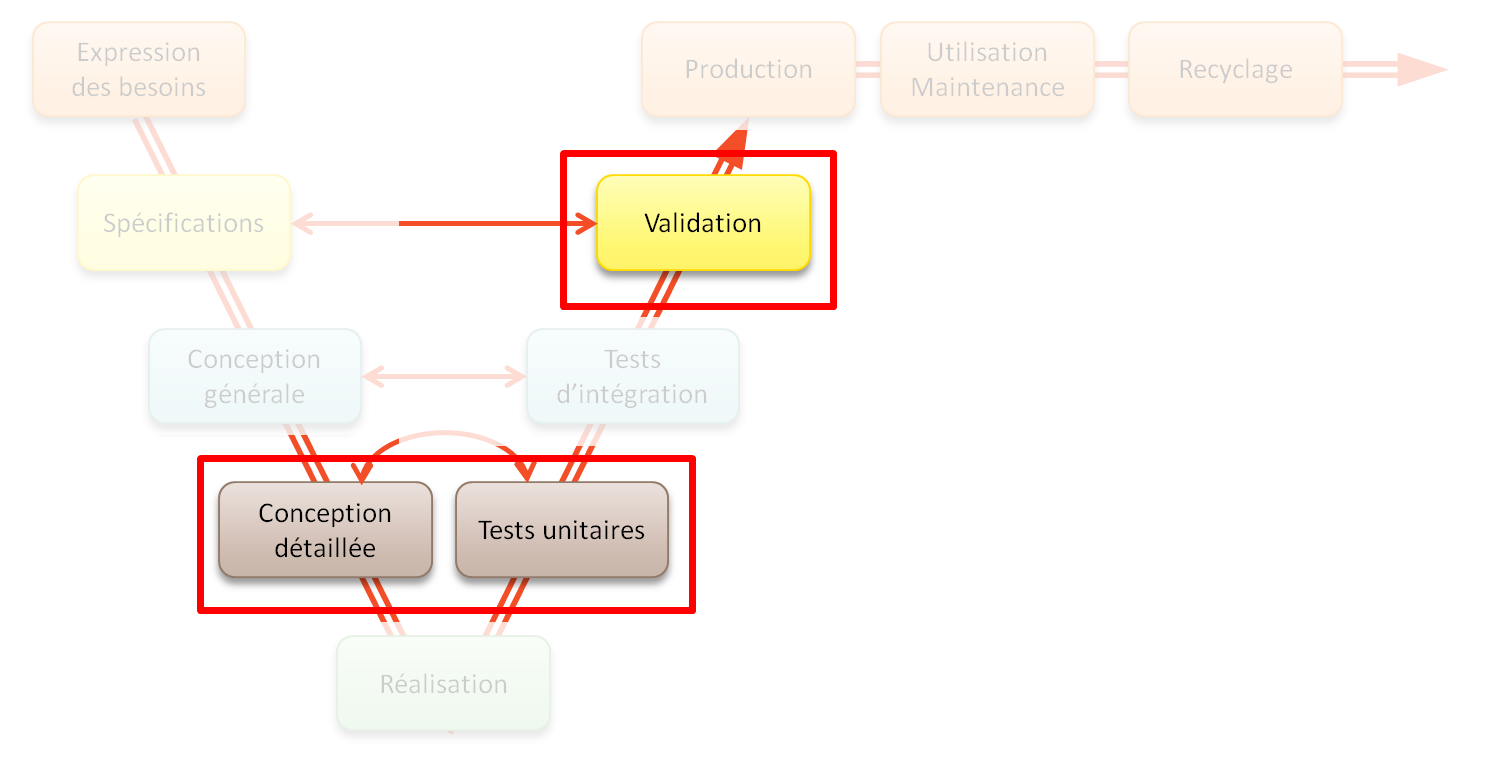
\includegraphics[width=.9\textwidth]{png/cyclev.png}

%\textit{Cycle de conception d'un produit}
%\end{center}

%\begin{prob}
%\textsc{Problématique :}

%En phase d'avant conception d'un produit, quels sont les critères qui vont permettre de choisir les matériaux à utiliser ?
%\end{prob}



\begin{savoir}
\textsc{Savoirs :}
\begin{itemize}
\item Disposer des cotes sur un dessin de façon normalisée
%\item Lire et interpréter une spécification géométrique ou dimensionnelle
\end{itemize}
\end{savoir}
 

\setlength{\parskip}{0ex plus 0.2ex minus 0ex}
 \renewcommand{\contentsname}{}
 \renewcommand{\baselinestretch}{1}

\tableofcontents

 \renewcommand{\baselinestretch}{1.2}
\setlength{\parskip}{2ex plus 0.5ex minus 0.2ex}

% \vspace{1cm}
\textit{Ce document évolue. Merci de signaler toutes erreurs ou coquilles.}




\section{Spécifications dimensionnelles des arbres et des moyeux}

On a vu que les spécifications dimensionnelles sur les arbres ou sur les moyeux pouvaient être représentés ainsi : 

\begin{center}
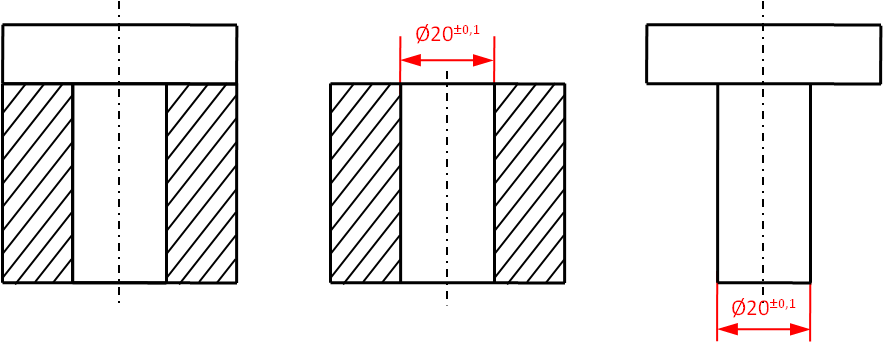
\includegraphics[width=.9\textwidth]{png/fig1.png}
\end{center}

Notons $D$ le diamètre de l'alésage et $d$ le diamètre de l'arbre. Dans ces conditions dimensionnelles, si on fabrique un arbre au diamètre le plus petit et un alésage au diamètre le plus grand on aura $d = 19,9\, mm$ et $D = 20,1\, mm$. Le jeu entre les deux pièces sera donc de 0,2 mm. L'assemblage des deux composants ne posera donc pas de problèmes.

Si on fabrique un arbre au diamètre le plus grand et un alésage au diamètre le plus petit on aura $d = 20,1\, mm$ et $D = 19,9\, mm$. Le jeu entre les deux pièces sera donc de -0,2 mm. L'assemblage des deux composants est maintenant plus difficile. 

\subsection{Vocabulaire}

\begin{center}
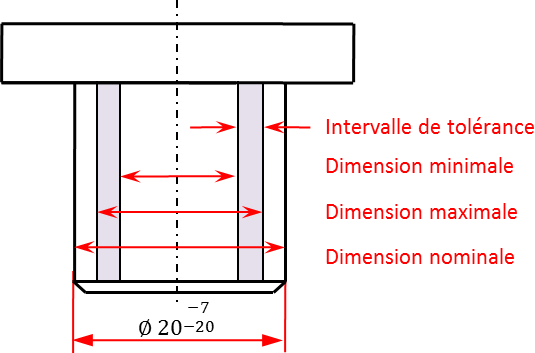
\includegraphics[width=.6\textwidth]{png/voca}
\end{center}


\begin{defi}
Lors de l'écriture de $\phi 20^{\begin{array}{c}-7 \\ -20 \end{array}}$ on appelle : 
\begin{itemize}
\item $\phi 20$ : la cote nominale;
\item l'intervalle de tolérance (\textbf{IT}) est de $13\mu m$;
\item l'écart supérieur (\textbf{ES}) est de $7\mu m$;
\item l'écart inférieur (\textbf{EI}) est de $20\mu m$.
\end{itemize}
\end{defi}

\subsection{Désignation des tolérances}
Usuellement, les intervalles de tolérances sont choisis dans une gamme normalisée. 
La représentation utilisée est la suivante : 
\begin{center}
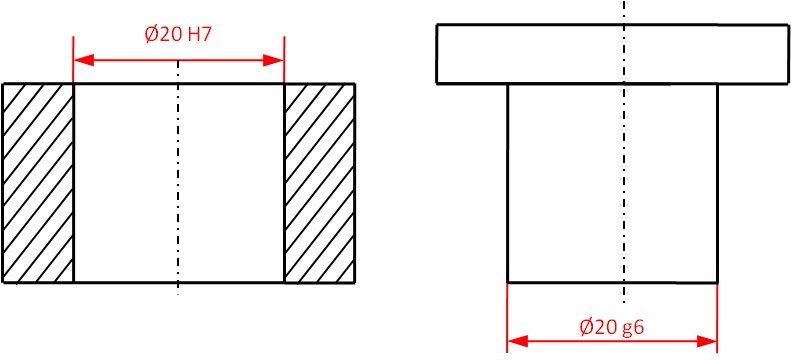
\includegraphics[width=.8\textwidth]{png/fig2.png}
\end{center}


\begin{resultat}
Les arbres sont côtés avec des lettres en minuscules de $a$ à $z$. 
Les moyeux sont côtés avec des lettres majuscules de $A$ à $Z$. 
Ces lettres définissent la position de l'intervalle de tolérance par rapport à la dimension nominale.

\vspace{1cm}

Le nombre suivant la lettre est appelé \textbf{degré de tolérance} et donne une indication de l'intervalle de tolérance. Plus la qualité est petite, plus l'intervalle de tolérance est petit. Plus la qualité est petite plus le prix est élevé.
\end{resultat}

\begin{minipage}[c]{.45\linewidth}
\begin{center}
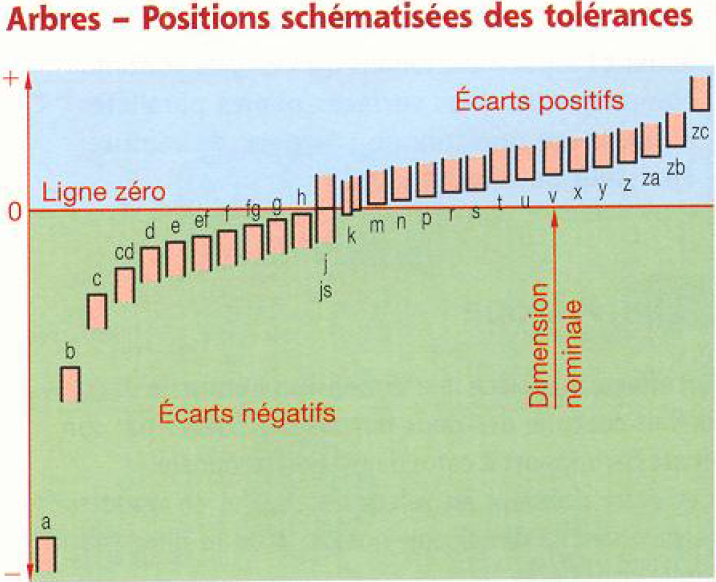
\includegraphics[width=.9\textwidth]{png/arbre}
\end{center}

Un arbre tolérancé avec une lettre "inférieure" à \textbf{h} aura toujours une dimension \textbf{inférieure} à la dimension nominale.

Un arbre tolérancé avec une lettre "supérieure" à \textbf{m} aura toujours une dimension \textbf{supérieure} à la dimension nominale.

Un arbre tolérancé avec la lettre \textbf{h} est toujours du type $\phi\; d ^{+0 / -x}$. C'est à dire qu'au maximum, le diamètre de l'arbre sera $d$.

\end{minipage}\hfill
\begin{minipage}[c]{.45\linewidth}
\begin{center}
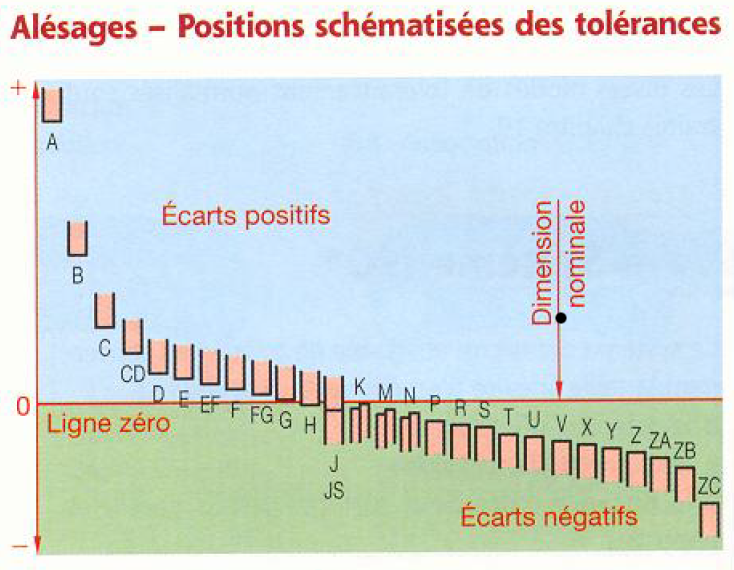
\includegraphics[width=.9\textwidth]{png/alesage}
\end{center}

Un alésage tolérancé avec une lettre "inférieure" à \textbf{H} aura toujours une dimension \textbf{supérieure} à la dimension nominale.

Un alésage tolérancé avec une lettre "supérieure" à \textbf{M} aura toujours une dimension \textbf{inférieure} à la dimension nominale.

Un alésage tolérancé avec la lettre \textbf{H} est toujours du type $\phi\; D ^{+x / -0}$. C'est à dire qu'au minimum, le diamètre de l'arbre sera $D$.
\end{minipage}

\begin{rem}
Plus le nombre sera petit plus l'intervalle de tolérance sera petit. En conséquence, la dimension sera plus difficile à fabriquer. Le coût de la pièce sera donc plus élevé. 
\end{rem}


\section{Spécification des assemblages}
La spécification des ajustements est utilisée pour coter les assemblages. Elle permet de savoir si le concepteur désire que deux pièces assemblées soient montées glissantes, serrées ou avec un jeu incertain.

\begin{exemple}
\begin{minipage}[c]{.3\linewidth}
\begin{center}
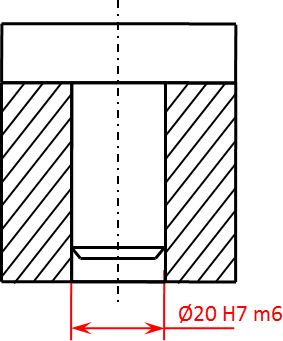
\includegraphics[width=.9\textwidth]{png/serre}

Ajustement serré
\end{center}

$$\phi 20 H7 = \phi 20^{+21/0} $$
$$ \phi 20 m6 = \phi 20^{+21/+8}$$

$$jeu_{mini}= -21\mu m $$
$$jeu_{max}=13\mu m$$

\end{minipage}\hfill
\begin{minipage}[c]{.3\linewidth}
\begin{center}
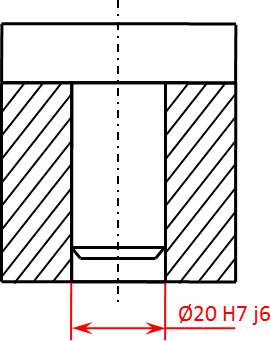
\includegraphics[width=.9\textwidth]{png/incertain}

Ajustement incertain
\end{center}

$$\phi 20 H7 = \phi 20^{+21/0} $$
$$\phi 20 j6 = \phi 20^{+9/-4}$$

$$jeu_{mini}= -9\mu m$$
$$jeu_{max}=25\mu m$$

\end{minipage}\hfill
\begin{minipage}[c]{.3\linewidth}
\begin{center}
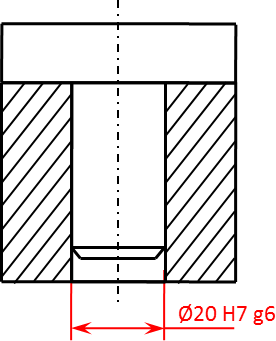
\includegraphics[width=.9\textwidth]{png/glissant}

Ajustement glissant
\end{center}

$$\phi 20 H7 = \phi 20^{+21/0} $$
$$\phi 20 g6 = \phi 20^{-7/-20}$$

$$jeu_{mini}= 7\mu m$$
$$jeu_{max}=41\mu m$$
\end{minipage}
\end{exemple}

\begin{rem}
En fabrication, il est plus facile de fabriquer des pièces "extérieures" (comme des arbres) que des pièces "intérieures" comme les moyeux. En conséquence, l'intervalle de tolérance sera plus grand sur les moyeux que sur les arbres. 

Cela se traduit par le fait que le degré de qualité est supérieur sur le moyeu que sur l'arbre (et donc que l'intervalle de tolérance est plus élevé sur le moyeu que sur l'arbre).
\end{rem}


%\subsection{Exigences particulières}

%\section{États de surface}

%\section{Métrologie}

%\section{Démarche de cotation fonctionnelle}

%\section{Ajustements}

%\section{Chaînes de cotes}


\begin{thebibliography}{2}
\bibitem{gdi}{\textit{Guide du dessinateur industriel}, André Chevalier, Éditions Hachette Technique, Editions 2004.}
%\bibitem{gps}{\textit{Centre d'Études et de Rénovation Pédagogique de l'Enseignement Technique}, Exploitation du concept G.P.S. et de la normalisation pour la Spécification Géométrique des Produits.}
%\bibitem{gps2}{\textit{Le Décodage du Dessin de Définition}, Guy Percebois, Lycée Louis Vincent -- Metz . \url{http://www.ac-nancy-metz.fr/enseign/sti/genimeca/zip/GPS/Tol\%20g\%E9o\%20pr\%E9\%20bac.pdf}}
%\bibitem{rb}{Supports de cours de Renan Bonnard,PTSI, Lycée Newton, Clichy la Garenne}
%\bibitem{jb}{Supports de cours de Joël Boiron, PTSI, Lycée Gustave Eiffel, Bordeaux}
%\bibitem{mc}{Supports de cours de Maryline Carrez, Lycée Jules Haag, Besançon}
%\bibitem{pf}{Supports de cours de Philippe Fichou, Lycée Vauban, Brest \url{http://philippe.fichou.pagesperso-orange.fr/documents/liaisoncomplete2003.pdf}}
%\bibitem{jpp}{Supports de cours de Jean-Pierre Pupier, Lycée Rouvière, Toulon}


\end{thebibliography}

\end{document}